\chapter{Background}
\label{cha:background}

\section{Gaussian Processes}
In \cite{Rasmussen2004} everything we need to know about Gaussian Processes (GP) is written, good huh? \todo{Obviously edit this and fill out the section!}

\section{Combining GPs}
\todo{...}

\section{Exploratory Data Analysis}
Exploratory Data Analysis (EDA) is a broad concept containing various techniques \cite{Anselin1999, Gelman2003, Hoaglin2003, Tukey1977, Velleman1981} for exploring and analysing data.
Early popular techniques include \emph{box plots} and \emph{stem-and-leaf} displays.
A stem-and-leaf plot takes numbers and splits them into two groups.
The first group contains the leading digit(s) and the second group contains the trailing digit(s).
Figure \ref{fig:stem-leaf-plot} is an example of a stem-and-leaf plot with one leading and one trailing digit.
The grouping helps when sorting batches of data and visualising important features, without losing the information of every single data point used \cite{Velleman1981}.

\begin{figure} [h!]
    \centering
    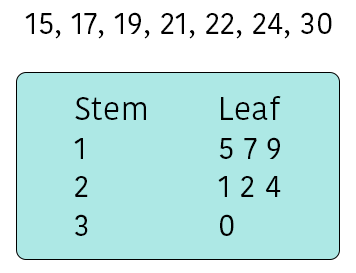
\includegraphics[width=0.33\textwidth]{figures/stem-leaf-plot}
    \caption{Example of a stem-and-leaf plot. The numbers above the plot is the input.
    The first digit of the number is the \emph{stem}, the following digits are the \emph{leafs}.}
    \label{fig:stem-leaf-plot}
\end{figure}

EDA can be seen as applying tools and statistics to analyse data in a meaningful way, e.g., it could be applied to the detection of outliers, smoothing the data, and performing a variance analysis \cite{Anselin1999, Hoaglin2003, Tukey1977, Velleman1981}.
EDA can also reveal subtle practical problems with the chosen model that can easily be missed when performing statistical theory analysis of the model \cite{Gelman2003}.

In \cite{Tukey1977}, Tukey describes how EDA can be used to answer research questions such as "What is the age distribution for the Vietnamese population?" and "Are there differences in
the annual household per capita expenditures between the rural and urban populations in Vietnam?".
Tukey uses plots to compare different groups and estimators to quantify the difference.
For example, the sample mean estimator, or the \emph{winsorised} mean can be used \cite{Tukey1977}.
The winsorised mean handles the case where tails of a distribution dominates the value space.  
This would cause the sample mean estimator to poorly reflect on the "typical" data point, as it is skewed by the small tail population \cite{Tukey1977}.

In \cite{Velleman1981}, Velleman et al. present different EDA techniques and highlights four key areas of EDA: displays (plots), residuals, re-expressions and resistance.
Residuals is what remains after data analysis is performed.
Residuals could, for example, be what remains after fitting data to a model (the error of the fit) \cite{Velleman1981}.
Re-expression is the notion of applying mathematical functions to the data.
Re-expressing the data can help with the data analysis \cite{Hoaglin2003, Velleman1981}.
Examples of mathematical functions that can be applied are: logarithm, square root, reciprocal square function or generally raising the data to some power $p$.
Resistance is the concept that outliers should not disproportionately affect the data analysis \cite{Hoaglin2003, Velleman1981}.
For example, the winsorised mean estimator would be less sensitive to localised misbehaviour than the sample mean estimator \cite{Tukey1977}.

Smoothing data is important for many different applications \cite{Bradley1997, Pang2002, Quinlan1992, Velleman1981}.
This can, for example, be done by applying \emph{running median smoothers}.
The running median smoothers go through all the data points in sequence and calculate only the median for the $n$ closest values near each point \cite{Velleman1981}.
Another approach is the \emph{running weighted average} \cite{Velleman1981}.
Instead of taking the median of the $n$ values, the average is calculated.
The average can also be weighted with different functions, like hanning smoothing \cite{Velleman1981}.
The hanning smoothing for three data points is shown in Eq. \ref{eq:hanning}.
It is worth noting that a single outlier will heavily affect the hanning smoothing and that in practice it is common to first apply a running median smoothing to remove outliers \cite{Velleman1981}.

\begin{equation}
    \hat y_t = \frac{1}{4} y_{t-1} + \frac{1}{2} y_t + \frac{1}{4} y_{t + 1} 
    \label{eq:hanning}
\end{equation}